\documentclass[11pt,a4paper]{article}
\input{../../sablony/pripravy/priprava.sty}
\usepackage{tikz,pgfplots}
\pgfplotsset{compat=1.18}
\nastavPripravu{1. ročník}{Kvadratické rovnice a nerovnice}{115}{Kvadratické rovnice s absolutní hodnotou II}
\begin{document}
\blok{Kvadratické rovnice s absolutní hodnotou II}
Modul u neznámé, rozdíl $|q(x)|$ versus $q(|x|)$, souměrnost podle osy $y$.
\blok{Metoda a návaznost na graf}
\poznamka{U každého přechodu odmocněním platí $\sqrt{u^2}=|u|$, nikoli obecně $u$. Závěrečný graf ověřuje i platnost intervalových podmínek.}
\begin{itemize}
\item U funkce $q(|x|)$ převezmi část grafu $q(x)$ pro $x\ge0$ a zrcadli ji podle osy $y$.
\item Polož $t=|x|\ge0$, vyřeš rovnici pro $t$, potom obnov obě znaménka $x$.
\item Pozor: $|x|^2=x^2$, ale $-4|x|\ne-4x$ pro záporná $x$.
\end{itemize}
\blok{Tabulka: modul u neznámé}
\begin{center}\renewcommand{\arraystretch}{1.26}\small
\begin{tabular}{@{}lcc@{}}\toprule
$x$ & $(-\infty;0)$ & $(0;+\infty)$\\\midrule
$|x|$ & $-(x)$ & $+(x)$\\\midrule
$y=x^2-4|x|+3$ & $x^2+4x+3$ & $x^2-4x+3$\\\bottomrule
\end{tabular}
\end{center}
\poznamka{V bodě $x=0$ mají oba předpisy shodnou hodnotu; graf je spojitý, ale může mít ostrý zlom.}

\begin{center}
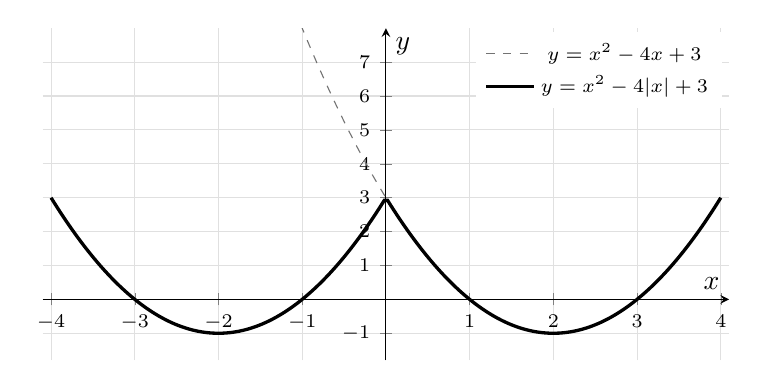
\begin{tikzpicture}
\begin{axis}[width=10.3cm,height=5.8cm,xmin=-4.1,xmax=4.1,ymin=-1.8,ymax=8,
axis lines=middle,grid=both,grid style={black!12},minor tick num=0,xlabel={$x$},ylabel={$y$},
xtick={-4,-3,-2,-1,0,1,2,3,4},ytick={-1,0,1,2,3,4,5,6,7},
tick label style={font=\scriptsize},legend style={font=\scriptsize,draw=none,at={(.99,.99)},anchor=north east}]
\addplot[black!55,dashed,domain=-4:4,samples=180] {x^2-4*x+3};
\addlegendentry{$y=x^2-4x+3$}
\addplot[black,very thick,domain=-4:4,samples=200,restrict y to domain=-2:8] {x^2-4*abs(x)+3};
\addlegendentry{$y=x^2-4|x|+3$}
\end{axis}
\end{tikzpicture}
\end{center}
\poznamka{Tady neobracíme graf podle osy $x$. Vezmeme pravou část a zrcadlíme podle osy $y$.}
\blok{Společně řešené příklady}
\begin{prikladReseniBox}[title={Příklad 1}]
$x^{2} - 4 \cdot \left|{x}\right| + 3=0$
\tcblower
\[
\begin{aligned}
t&=|x|\ge0\\[2pt]
t^{2} - 4 \cdot t + 3&=0\quad\text{(řešíme pro }t\text{)}\\[2pt]
t&\in \{1;3\}\\[2pt]
K&=\{-3;-1;1;3\}
\end{aligned}
\]
\end{prikladReseniBox}
\begin{prikladReseniBox}[title={Příklad 2}]
$x^{2} - 4 \cdot \left|{x}\right| + 4=0$
\tcblower
\[
\begin{aligned}
t&=|x|\ge0\\[2pt]
t^{2} - 4 \cdot t + 4&=0\quad\text{(řešíme pro }t\text{)}\\[2pt]
t&\in \{2\}\\[2pt]
K&=\{-2;2\}
\end{aligned}
\]
\end{prikladReseniBox}
\begin{prikladReseniBox}[title={Příklad 3}]
$x^{2} - 2 \cdot \left|{x}\right| - 3=0$
\tcblower
\[
\begin{aligned}
t&=|x|\ge0\\[2pt]
t^{2} - 2 \cdot t - 3&=0\quad\text{(řešíme pro }t\text{)}\\[2pt]
t&\in \{3\}\\[2pt]
K&=\{-3;3\}
\end{aligned}
\]
\end{prikladReseniBox}
\blok{Samostatné procvičování}
\begin{zadaniReseniBox}[title={Úloha 1}]
$x^{2} - 6 \cdot \left|{x}\right| + 8=0$
\tcblower
\[
\begin{aligned}
t&=|x|\ge0\\[2pt]
t^{2} - 6 \cdot t + 8&=0\quad\text{(řešíme pro }t\text{)}\\[2pt]
t&\in \{2;4\}\\[2pt]
K&=\{-4;-2;2;4\}
\end{aligned}
\]
\end{zadaniReseniBox}
\begin{zadaniReseniBox}[title={Úloha 2}]
$x^{2} + 2 \cdot \left|{x}\right| - 3=0$
\tcblower
\[
\begin{aligned}
t&=|x|\ge0\\[2pt]
t^{2} + 2 \cdot t - 3&=0\quad\text{(řešíme pro }t\text{)}\\[2pt]
t&\in \{1\}\\[2pt]
K&=\{-1;1\}
\end{aligned}
\]
\end{zadaniReseniBox}
\blok{Volitelná grafická rezerva}
Srovnejte grafy $y=x^2-4|x|+3$ a $y=|x^2-4x+3|$. Proč nejsou stejné?
\blok{Další možnost -- když modul není jen u $x$}
\begin{zadaniReseniBox}[title={Rozšiřující příklad}]
Načrtněte $y=|x(x-3)|$ a porovnejte s $y=|x|(x-3)$. Jsou grafy stejné?
\tcblower
\[\begin{aligned}
|x(x-3)|&=\begin{cases}x(x-3),&x\le0\ \text{nebo}\ x\ge3,\\-x(x-3),&0<x<3,\end{cases}\\|x|(x-3)&=\begin{cases}-x(x-3),&x<0,\\x(x-3),&x\ge0.\end{cases}\\\text{Grafy nejsou stejné.}&
\end{aligned}\]
\end{zadaniReseniBox}
\blok{Domácí úkol}
\begin{zadaniReseniBox}[title={Domácí příprava}]
\begin{enumerate}[label=\alph*),itemsep=2pt]
\item $x^{2} - 4 \cdot \left|{x}\right|=0$
\item $x^{2} - 6 \cdot \left|{x}\right| + 5=0$
\item $x^{2} - 2 \cdot \left|{x}\right|=0$
\item $x^{2} - 8 \cdot \left|{x}\right| + 12=0$
\item $x^{2} + 4 \cdot \left|{x}\right| + 3=0$
\item $x^{2} - 4 \cdot \left|{x}\right| - 5=0$
\end{enumerate}
\tcblower
\begin{enumerate}[label=\alph*),itemsep=2pt]
\item
\[\begin{aligned}
t&=|x|\ge0\\[2pt]
t^{2} - 4 \cdot t&=0\quad\text{(řešíme pro }t\text{)}\\[2pt]
t&\in \{0;4\}\\[2pt]
K&=\{-4;0;4\}
\end{aligned}\]
\item
\[\begin{aligned}
t&=|x|\ge0\\[2pt]
t^{2} - 6 \cdot t + 5&=0\quad\text{(řešíme pro }t\text{)}\\[2pt]
t&\in \{1;5\}\\[2pt]
K&=\{-5;-1;1;5\}
\end{aligned}\]
\item
\[\begin{aligned}
t&=|x|\ge0\\[2pt]
t^{2} - 2 \cdot t&=0\quad\text{(řešíme pro }t\text{)}\\[2pt]
t&\in \{0;2\}\\[2pt]
K&=\{-2;0;2\}
\end{aligned}\]
\item
\[\begin{aligned}
t&=|x|\ge0\\[2pt]
t^{2} - 8 \cdot t + 12&=0\quad\text{(řešíme pro }t\text{)}\\[2pt]
t&\in \{2;6\}\\[2pt]
K&=\{-6;-2;2;6\}
\end{aligned}\]
\item
\[\begin{aligned}
t&=|x|\ge0\\[2pt]
t^{2} + 4 \cdot t + 3&=0\quad\text{(řešíme pro }t\text{)}\\[2pt]
t&\in \varnothing\\[2pt]
K&=\varnothing
\end{aligned}\]
\item
\[\begin{aligned}
t&=|x|\ge0\\[2pt]
t^{2} - 4 \cdot t - 5&=0\quad\text{(řešíme pro }t\text{)}\\[2pt]
t&\in \{5\}\\[2pt]
K&=\{-5;5\}
\end{aligned}\]
\end{enumerate}
\end{zadaniReseniBox}
\poznamka{Orientační čas: úvod 5 min, společné příklady 18 min, samostatně 15 min, kontrola a shrnutí 7 min. Rezerva je dobrovolná. Číselné parametry modelových aplikací nejsou skutečně naměřená data.}
\end{document}
